\documentclass[12pt, letterpaper, twoside]{article}

\usepackage{geometry}
\usepackage{graphicx}
\usepackage{amsmath, amsfonts, amssymb, bbm}
%\usepackage{lipsum}
\usepackage{fancyhdr}
%\usepackage{layout}
\usepackage{lettrine}
\usepackage[explicit]{titlesec}
\usepackage{hyperref}
\usepackage{watermark}
\usepackage{color}

%%%%%%%%%%%%%%%%%%%%%%%% 
% FONT SELECTION  
%%%%%%%%%%%%%%%%%%%%%%%% 

\usepackage[light,math]{iwona}
\usepackage[T1]{fontenc}

%%%%%%%%%%%%%%%%%%%%%%%%
% DEFINE COLORS
%%%%%%%%%%%%%%%%%%%%%%%%

\definecolor{grey}{rgb}{0.5,0.5,0.5}
\definecolor{l-grey}{rgb}{0.8,0.8,0.8}
\definecolor{withe}{rgb}{1,1,1}
\definecolor{black}{rgb}{0,0,0}

%%%%%%%%%%%%%%%%%%%%%%%% 
% PAGE LAYOUT
%%%%%%%%%%%%%%%%%%%%%%%%

% Paper Width 614pt
% Text fill symemetric 604pt
% Paper Height 794pt

\setlength{\voffset}{-0.5in}
\setlength{\hoffset}{-1in}
\setlength{\oddsidemargin}{65pt}
\setlength{\evensidemargin}{45pt}
\setlength{\topmargin}{0in}
\setlength{\headheight}{15pt}
\setlength{\headsep}{20pt}
\setlength{\marginparwidth}{0in}
\setlength{\marginparsep}{0in}
\setlength{\textheight}{635pt}
\setlength{\textwidth}{494pt}
\setlength{\footskip}{50pt}

%%%%%%%%%%%%%%%%%%%%%%%%
% TITLES LAYOUT
%%%%%%%%%%%%%%%%%%%%%%%%

\titleformat{\section}[display]
{\vspace*{150pt}
\bf\Huge}
{\begin{picture}(0,0)\put(-60,-30){\textcolor{grey}{\thesection}}\end{picture}}
{0pt}
{#1}
[]

% initial margin, ????, bottom margin final margin
\titlespacing*{\section}{40pt}{10pt}{40pt}[40pt]
\newcommand{\sectionbreak}{\cleardoublepage}


%%%%%%%%%%%%%%%%%%%%%%%%
% MATH OPERATORS AND 
% CUSTOM ENVIRONMENTS
%%%%%%%%%%%%%%%%%%%%%%%%
\DeclareMathOperator{\Tr}{Tr}
\DeclareMathOperator*{\Cov}{Cov}
\DeclareMathOperator{\cov}{Cov} 
  
\newcounter{observ}
\newenvironment{observ}{\refstepcounter{observ}
   \textit{\textbf{Observation \theobserv:}} \rmfamily}
     
\newenvironment{proof}{\textit{Proof:} \rmfamily}{\hfill$\square$}

\newcommand{\ket}[1]{\ensuremath{\vert #1 \rangle}}
\newcommand{\bra}[1]{\ensuremath{\langle #1 \vert}} 
\newcommand{\braket}[2]{\ensuremath{\langle #1 \vert #2 \rangle}} 
\newcommand{\braOket}[3]{\ensuremath{\langle #1 \vert #2 \vert #3 \rangle}}
\newcommand{\ketbra}[2]{\ensuremath{\vert #1 \rangle \! \langle #2 \vert}}
\newcommand{\meanO}[1]{\ensuremath{\langle #1 \rangle}}
\newcommand{\ver}[2]{\ensuremath{\genfrac{}{}{0pt}{}{#1}{#2}}}
\newcommand{\tr}[1]{\ensuremath{\Tr \lcua #1\rcua}}
\newcommand{\trsub}[2]{\ensuremath{\Tr_{#1} \lcua #2 \rcua }}
\newcommand{\bsym}[1]{\ensuremath{\boldsymbol{#1}}}

\def\be{\begin{equation}}
\def\ee{\end{equation}}
\def\bea{\begin{eqnarray}}
\def\eea{\end{eqnarray}}
\def\bse{\begin{subequations}} 
\def\ese{\end{subequations}}
\def\mtxid{\mathbbm{1}}
\def\lpar{\left(} 
\def\rpar{\right)}
\def\lcua{\left[}
\def\rcua{\right]}
\def\lcor{\left\{}
\def\rcor{\right\}}
\def\lang{\left\langle}
\def\rang{\right\rangle}
\def\l{\left} 
\def\r{\right}
\def\nnnl{\nonumber\\}
\def\nnnlq{\nonumber\\ && \quad}
\def\nnnlqq{\nonumber\\ && \qquad}
\def\nnnlqqq{\nonumber\\ && \quad\qquad}
\def\ie{, \textit{i.e.}, }

%%%%%%%%%%%%%%%%%%%%%%%%
% DOCUMENT
%%%%%%%%%%%%%%%%%%%%%%%%
\begin{document}

\pagestyle{fancy}
\renewcommand{\sectionmark}[1]{\markboth{}{\MakeUppercase{\emph{#1}}}}
\renewcommand{\subsectionmark}[1]{\markboth{\emph{#1}}{}}
\renewcommand{\headrulewidth}{0pt}
\fancyhead{}
\fancyfoot{}

%%%%%%%%%%%%%%%%%%%%%%%%
% TITLE PAGE
%%%%%%%%%%%%%%%%%%%%%%%%

%!TEX root = main.tex 

\thiswatermark{\centering
\put(0,-110){
\includegraphics[height=2.5cm]{img/0-Ztf.png}} 
\put(430,-100){
\includegraphics[height=2cm]{img/0-Ehu.png}}
} 

\begin{center}

\vspace*{20pt}
\textsc{\LARGE University of the Basque Country}

\vspace{20pt}
\textsc{\Large PhD Thesis}

\vspace{50pt} 
\hrule 

\vspace{16pt}
{\huge \bfseries Lower bounds on quantum metrological precisions}
\vspace{16pt}

\hrule
\vspace{40pt}

\begin{minipage}{0.4\textwidth}
\begin{flushleft} \large
\emph{Author:}


M. Sc. Iagoba \textsc{Apellaniz}
\end{flushleft}
\end{minipage}
\begin{minipage}{0.4\textwidth}
\begin{flushright} \large
\emph{Director:}

Prof. G\'eza \textsc{T\'oth} %TODO: Check Geza's name
\end{flushright}
\end{minipage}

\vspace{40pt}
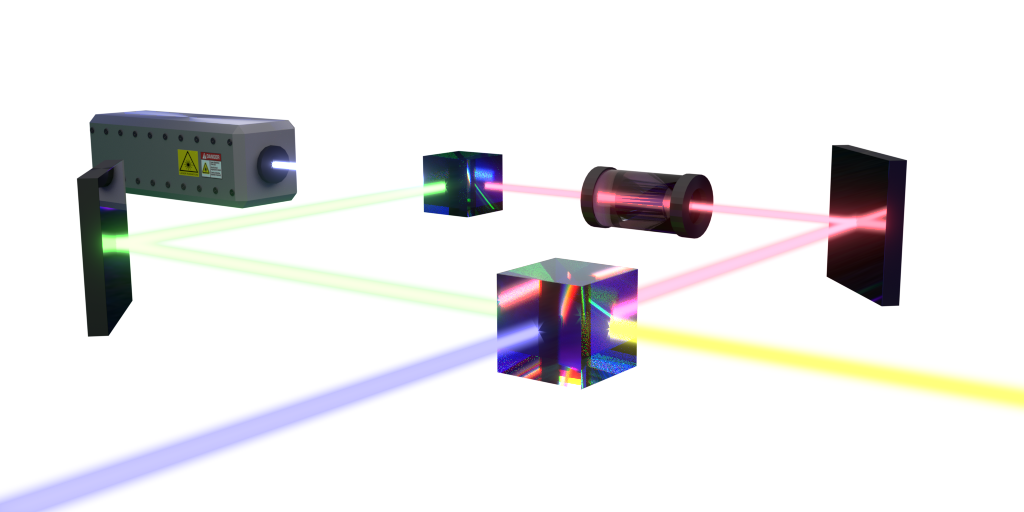
\includegraphics[width=0.8\hsize]{img/cover3Dpicture.png}
\vfill

% Bottom of the page
{\large \today}

\end{center}

\cleardoublepage

%%%%%%%%%%%%%%%%%%%%%%%%
% EDITION TIPS
%%%%%%%%%%%%%%%%%%%%%%%%

\cleardoublepage

This document was generated with the 2013 distribution of \LaTeX.

\vfill


\includegraphics[height=20pt]{img/0-CreativeCommons-by-sa.png}

2012-2014 Iagoba Apellaniz. This work is licensed under the Creative Commons
Attribution-ShareAlike 4.0 International License. To view a copy of this
license, visit
\href{http://creativecommons.org/licenses/by-sa/4.0/deed.en_US}
{http://creativecommons.org/ licenses/by-sa/4.0/deed.en\_US}.
\clearpage

%%%%%%%%%%%%%%%%%%%%%%%%
% PROLOGE
%%%%%%%%%%%%%%%%%%%%%%%%

\section*{Prologue}
\setcounter{page}{1}
\pagenumbering{roman}
\fancyfoot[LE,RO]{\thepage}

Here is the prologue.

%%%%%%%%%%%%%%%%%%%%%%%%
% TABLE OF CONTENTS
%%%%%%%%%%%%%%%%%%%%%%%%

\vspace*{100pt}
\tableofcontents

%%%%%%%%%%%%%%%%%%%%%%%%
% THESIS
%%%%%%%%%%%%%%%%%%%%%%%%

\cleardoublepage
\setcounter{page}{1}
\pagenumbering{arabic}
\fancyfoot{}
%!TEX root = main.tex 

\thiswatermark{\centering
\put(0,-110){
\includegraphics[height=2.5cm]{img/0-Ztf.png}} 
\put(430,-100){
\includegraphics[height=2cm]{img/0-Ehu.png}}
} 

\begin{center}

\vspace*{20pt}
\textsc{\LARGE University of the Basque Country}

\vspace{20pt}
\textsc{\Large PhD Thesis}

\vspace{50pt} 
\hrule 

\vspace{16pt}
{\huge \bfseries Lower bounds on quantum metrological precisions}
\vspace{16pt}

\hrule
\vspace{40pt}

\begin{minipage}{0.4\textwidth}
\begin{flushleft} \large
\emph{Author:}


M. Sc. Iagoba \textsc{Apellaniz}
\end{flushleft}
\end{minipage}
\begin{minipage}{0.4\textwidth}
\begin{flushright} \large
\emph{Director:}

Prof. G\'eza \textsc{T\'oth} %TODO: Check Geza's name
\end{flushright}
\end{minipage}

\vspace{40pt}
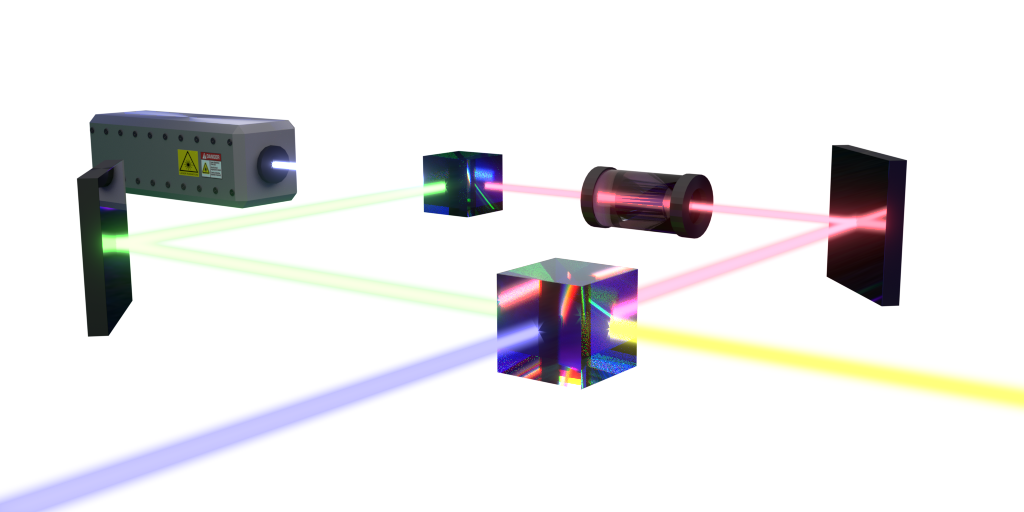
\includegraphics[width=0.8\hsize]{img/cover3Dpicture.png}
\vfill

% Bottom of the page
{\large \today}

\end{center}

\cleardoublepage
\cleardoublepage

%%%%%%%%%%%%%%%%%%%%%%%%
% DEDICATION PAGE
%%%%%%%%%%%%%%%%%%%%%%%%
\vspace*{100pt}
\begin{center}
\emph{To my parents and my family}
\end{center}

\cleardoublepage

%%%%%%%%%%%%%%%%%%%%%%%%
% HEADINGS AND PAGE NUM.
%%%%%%%%%%%%%%%%%%%%%%%%
\renewcommand{\headrulewidth}{0.5pt}
\fancyfoot[LE,RO]{\thepage}
\fancyhead[LE]{\rightmark}
\fancyhead[RO]{\leftmark}

%%%%%%%%%%%%%%%%%%%%%%%%
% REDEFINE TITLE FORMAT
%%%%%%%%%%%%%%%%%%%%%%%%
\titleformat{\section}[display]
{\vspace*{190pt}
\bf\Huge}
{\begin{picture}(0,0)\put(-64,-31){\textcolor{grey}{\thesection}}\end{picture}}
{0pt}
{\textcolor{withe}{#1}}
[]
\titlespacing*{\section}{100pt}{10pt}{40pt}[40pt]


\section{Introduction}
\thiswatermark{\put(1,-297){\color{l-grey}\rule{84pt}{42pt}}
\put(84,-297){\color{grey}\rule{410pt}{42pt}}}

\lettrine[lines=2, findent=3pt,nindent=0pt]{I}{n} recent years many work and
implementations of quantum metrology arise to the public domain.
The interest of this field is increasing day by day.

implementations of quantum metrology arise to the public domain.
The interest of this field is increasing day by day.

implementations of quantum metrology arise to the public domain.
The interest of this field is increasing day by day.
implementations of quantum metrology arise to the public domain.
The interest of this field is increasing day by day.

implementations of quantum metrology arise to the public domain.
The interest of this field is increasing day by day.
implementations of quantum metrology arise to the public domain.
The interest of this field is increasing day by day.
implementations of quantum metrology arise to the public domain.
The interest of this field is increasing day by day.

implementations of quantum metrology arise to the public domain.
The interest of this field is increasing day by day.
implementations of quantum metrology arise to the public domain.
The interest of this field is increasing day by day.
implementations of quantum metrology arise to the public domain.
The interest of this field is increasing day by day.
implementations of quantum metrology arise to the public domain.
The interest of this field is increasing day by day.
implementations of quantum metrology arise to the public domain.
The interest of this field is increasing day by day.

implementations of quantum metrology arise to the public domain.
The interest of this field is increasing day by day.
implementations of quantum metrology arise to the public domain.
The interest of this field is increasing day by day.
implementations of quantum metrology arise to the public domain.
The interest of this field is increasing day by day.
implementations of quantum metrology arise to the public domain.
The interest of this field is increasing day by day.

implementations of quantum metrology arise to the public domain.
The interest of this field is increasing day by day.

implementations of quantum metrology arise to the public domain.
The interest of this field is increasing day by day.
implementations of quantum metrology arise to the public domain.
The interest of this field is increasing day by day.
implementations of quantum metrology arise to the public domain.
The interest of this field is increasing day by day.


\section{Estimation processes}
\thiswatermark{\put(1,-297){\color{l-grey}\rule{84pt}{42pt}}
\put(84,-297){\color{grey}\rule{410pt}{42pt}}}

\lettrine[lines=2, findent=3pt,nindent=0pt]{I}{n} almost any area of science
and engineering the estimation process takes a fundamental role on 
data analysis.
So it is the importance that the estimation theory developed around has been 
studied since long time ago, reaching to a high level of complexity and 
to a rich functionality in terms of adaptability to a huge variety
of situations. 
In this chapter we will go trough the most important features of this
theory until reach transcendental concepts for the understandability of this
book. 

% line height 30pt
\section{Accuracy bound for gradient field estimation with atomic ensembles}
\thiswatermark{\put(1,-327){\color{l-grey}\rule{84pt}{72pt}}
\put(84,-327){\color{grey}\rule{410pt}{72pt}}} 


implementations of quantum metrology arise to the public domain.
The interest of this field is increasing day by day. 
implementations of quantum metrology arise to the public domain.
The interest of this field is increasing day by day.
implementations of quantum metrology arise to the public domain.
The interest of this field is increasing day by day.

implementations of quantum metrology arise to the public domain.
The interest of this field is increasing day by day.
implementations of quantum metrology arise to the public domain.
The interest of this field is increasing day by day.
implementations of quantum metrology arise to the public domain.
The interest of this field is increasing day by day.
implementations of quantum metrology arise to the public domain.
The interest of this field is increasing day by day.

\end{document}
